% !TEX TS-program = xelatex
% !TEX encoding = UTF-8 Unicode

\documentclass[11pt,tikz,border=1]{standalone}
\usepackage[default,mdseries=Light,bfseries=Medium,path=fonts]{cjkfonts}
\usepackage{pgfplots}
\usetikzlibrary{calc,pgfplots.colormaps}

\begin{document}
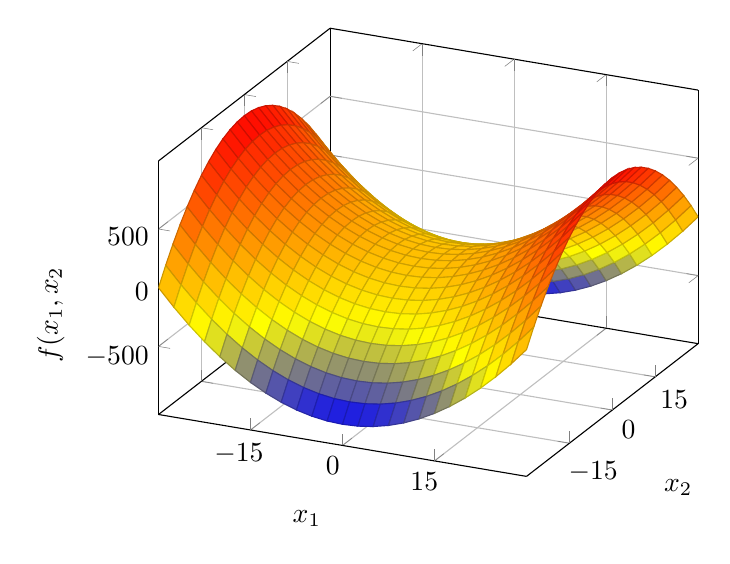
\begin{tikzpicture}

\begin{axis}[
  3d box=background,
  grid=major,
  xtick={-15,0,15},
  ytick={-15,0,15},
  ztick={-500,0,500},
  xlabel={$x_1$},
  ylabel={$x_2$},
  zlabel={$f(x_1,x_2$}
]

\addplot3[
  surf,
  domain=-30:30
]{
  x^2 - y^2
};  
  
\end{axis}

  
\end{tikzpicture}
\end{document}
